\chapterimage{chapterimage_1.jpg} % Chapter heading image

\chapter{Overview of the \ate{} UI and API}
\section{Introduction}\index{Introduction}

\doublespacing
This chapter gives an overview of the software application that is named \emph{ATExplorer}.

The \ate application was designed and implemented due to an emerging need to allow \emph{non-programmers} to process, manage and explore \at data on a routine basis.

Depending on the actual protocols, an \at data set can range in size from a few hundred megabytes, to very large, like several Terra bytes.  Depending on the number of stains and sessions, the complexity of the data-sets range from trivial to complex.

One of the main challenges in \at is the precise digital reconstruction of an original volume, i.e. from individually cut and imaged slices of tissue.

However, before volume reconstruction can begin, various pre data processing algorithms need to be applied, such as median filtering, flat-field correction and de-convolution. These processing algorithms are all, to some extent, complex. \ate provides the non-programmer user with intuitive and easy to use UI components to guide through this process, in order to quickly get to data that is useful for scientific discovery and exploration.

\section{A manual \at workflow}
In order to get from raw, acquired data to  fine aligned 3D volumes, a number of processing steps, i.e. a \emph{pipeline}, is required. (See pipeline figure)

\begin{description}[font=$\bullet$~\normalfont\scshape\color{red!50!black}]
\item [FlatField correction]
\item [Deconvolution]
\item [Stitching]
\item [Registration]
\item [Rough aligning] 
\item [Fine aligning] 
\item [Other]
\end{description}

The pipeline is integrated into the \ate UI. However, in certain situations it may be necessary to push data through the pipeline manually. \ate in ... provide a set of Python scripts that can be used for exactly this purpose. The scripts are to be found in the folder \path{/atPipeline/source} and \path{/atPipeline}. These scripts can be executed on their own, or from within the UI. 
each pipeline script is discussed in terms of their purpose, input and output data, in the sections below.

\subsection{Creation of \emph{state tables}}
\subsubsection{\emph{Fast stacks}}
Creates down-sampled images and tile specs...

\singlespacing
\begin{python}    
#------------------------------------------------
# Name:        atMain
# Purpose:     Run multiple AT processing scripts
#------------------------------------------------

import os
import atutils
import create_state_tables
import create_rawdata_render_multi_stacks
import create_median_files
import create_flatfield_corrected_data
import timeit

if __name__ == '__main__':
    timeStart = timeit.default_timer()

    #What data to process??
    dataRootFolder = "F:\\data\\M33"
    ribbons = ["Ribbon0004"]
    sessions = ["Session01",
                "Session02",
                "Session03"
                ]

\end{python}

\doublespacing

\subsection{Creation of median files}
\subsection{FlatField correction}

\clearpage

\begin{figure}[h]
\centering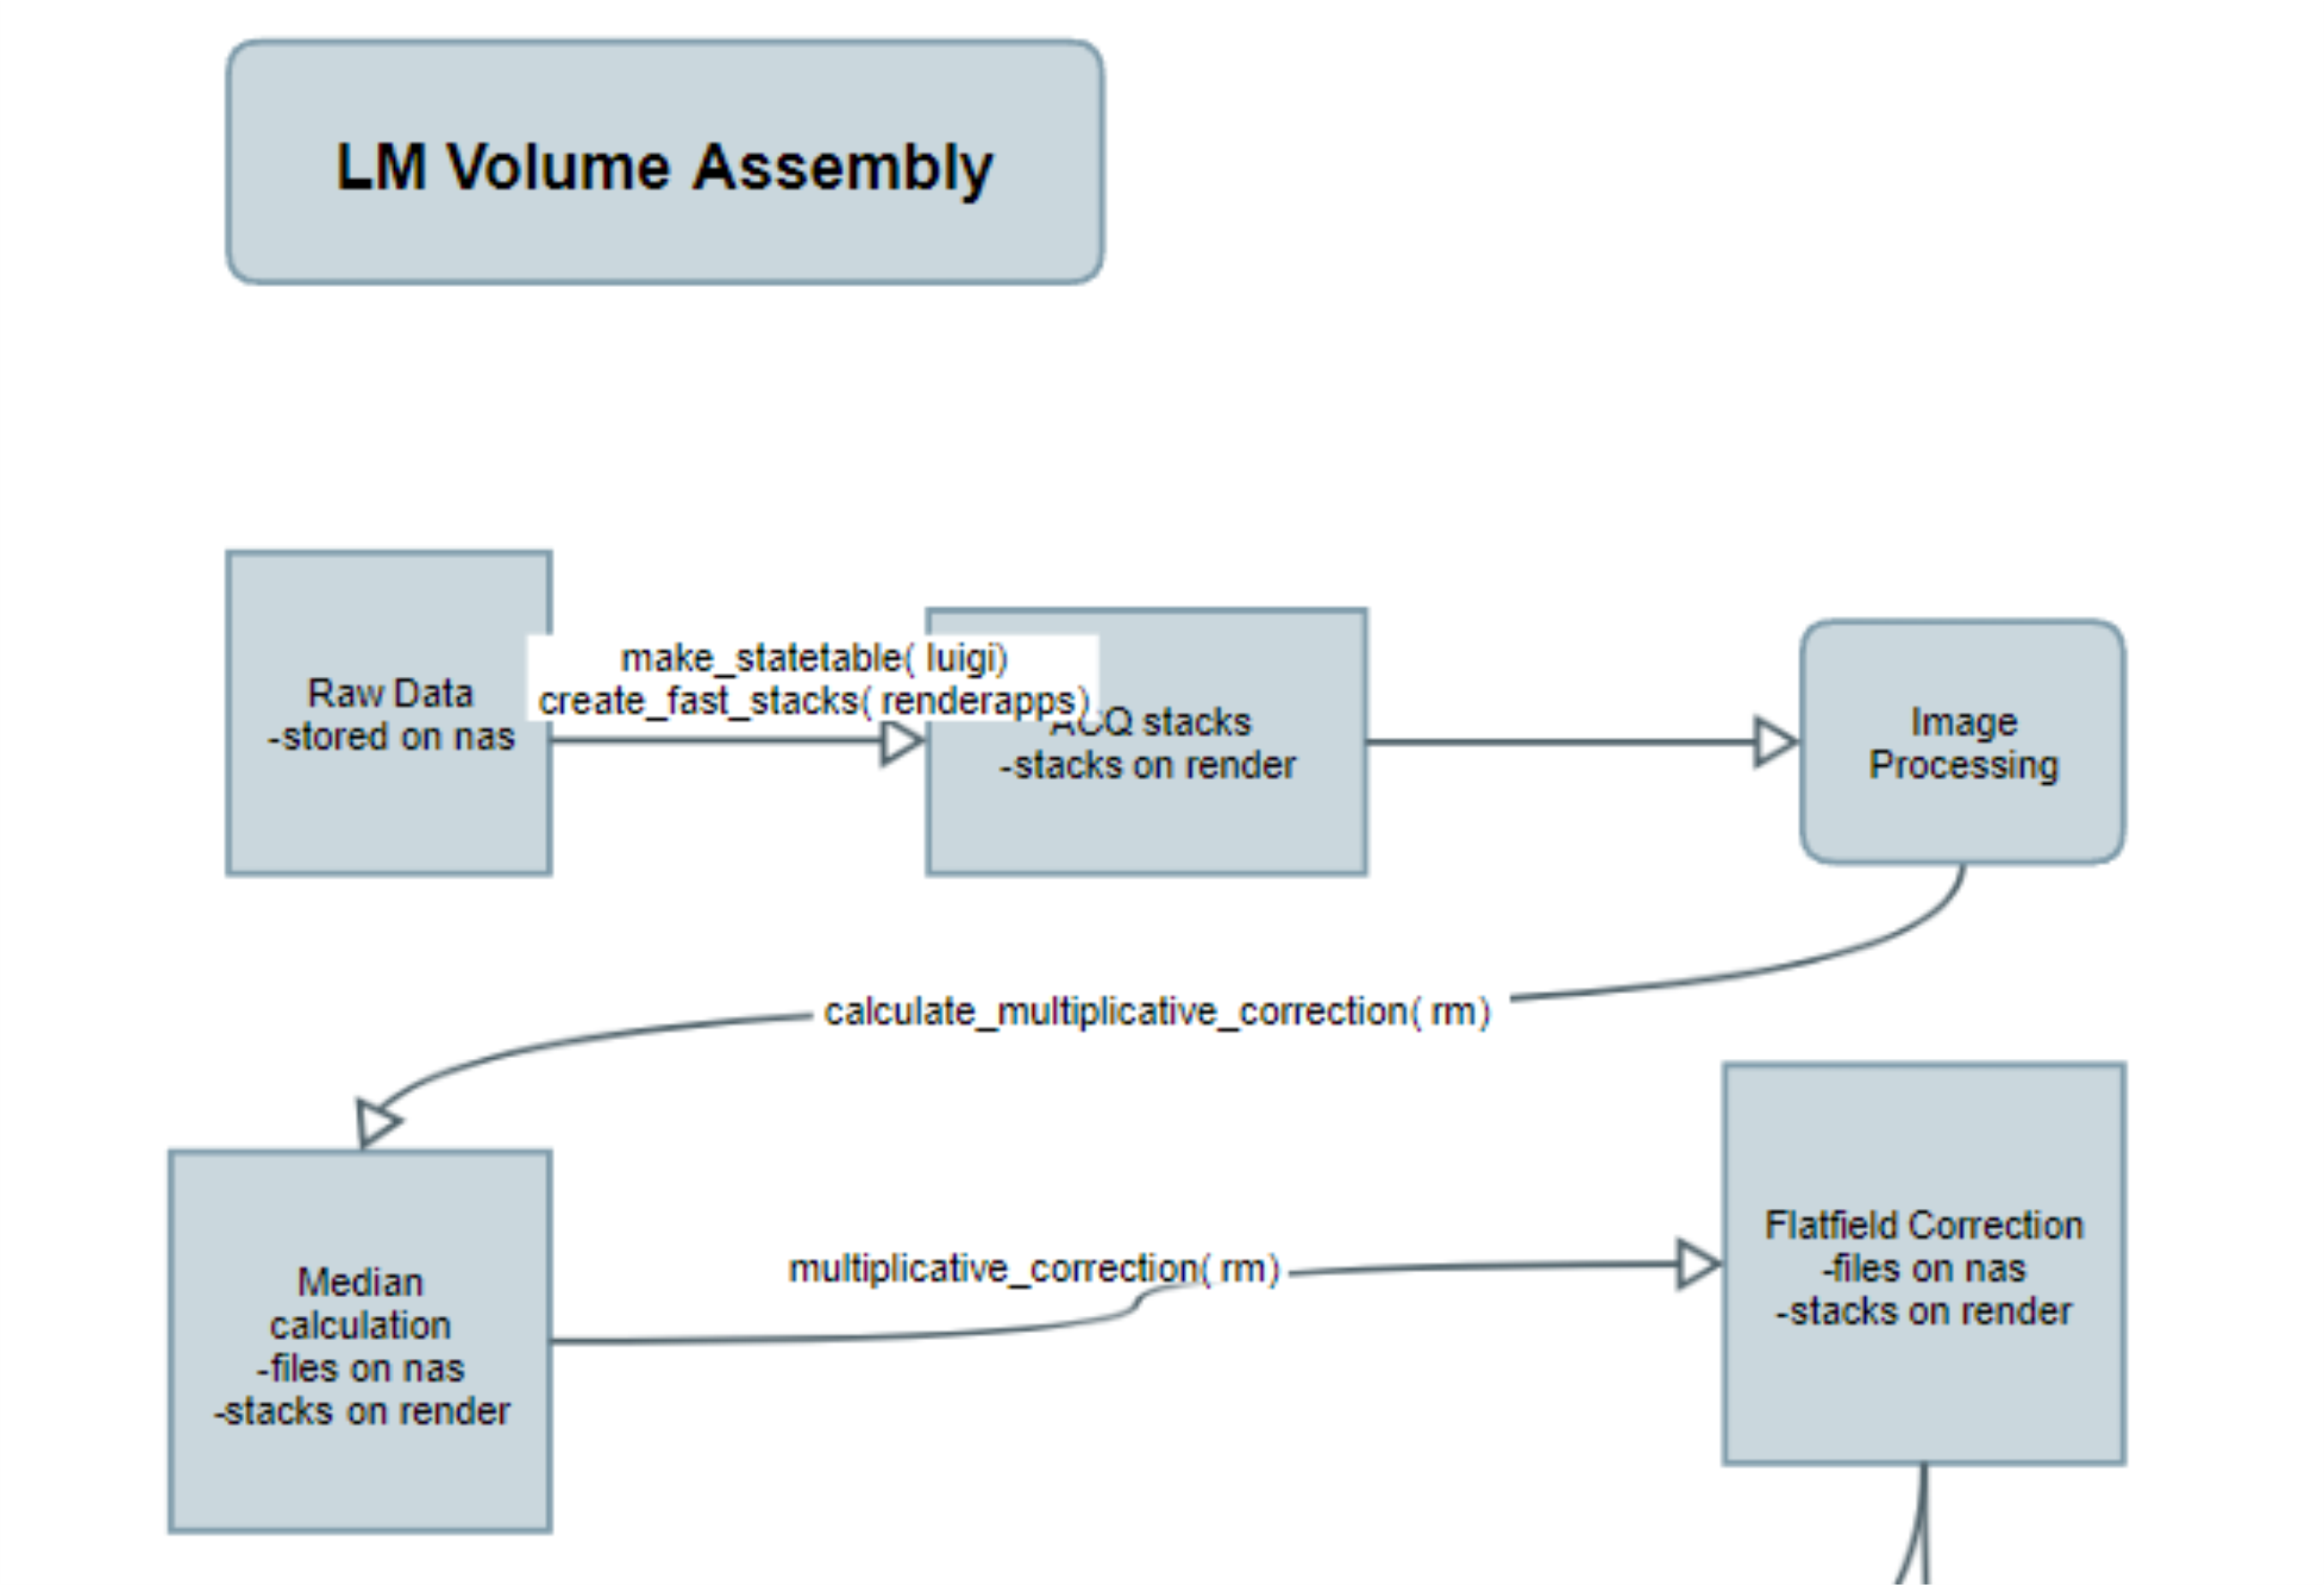
\includegraphics[scale=0.65]{LMDataProcessing_1}

\caption{Processing ..........}
\end{figure}

\section{The Render Service}

\clearpage

\section{The \ate UI}

\begin{figure}[h]
\centering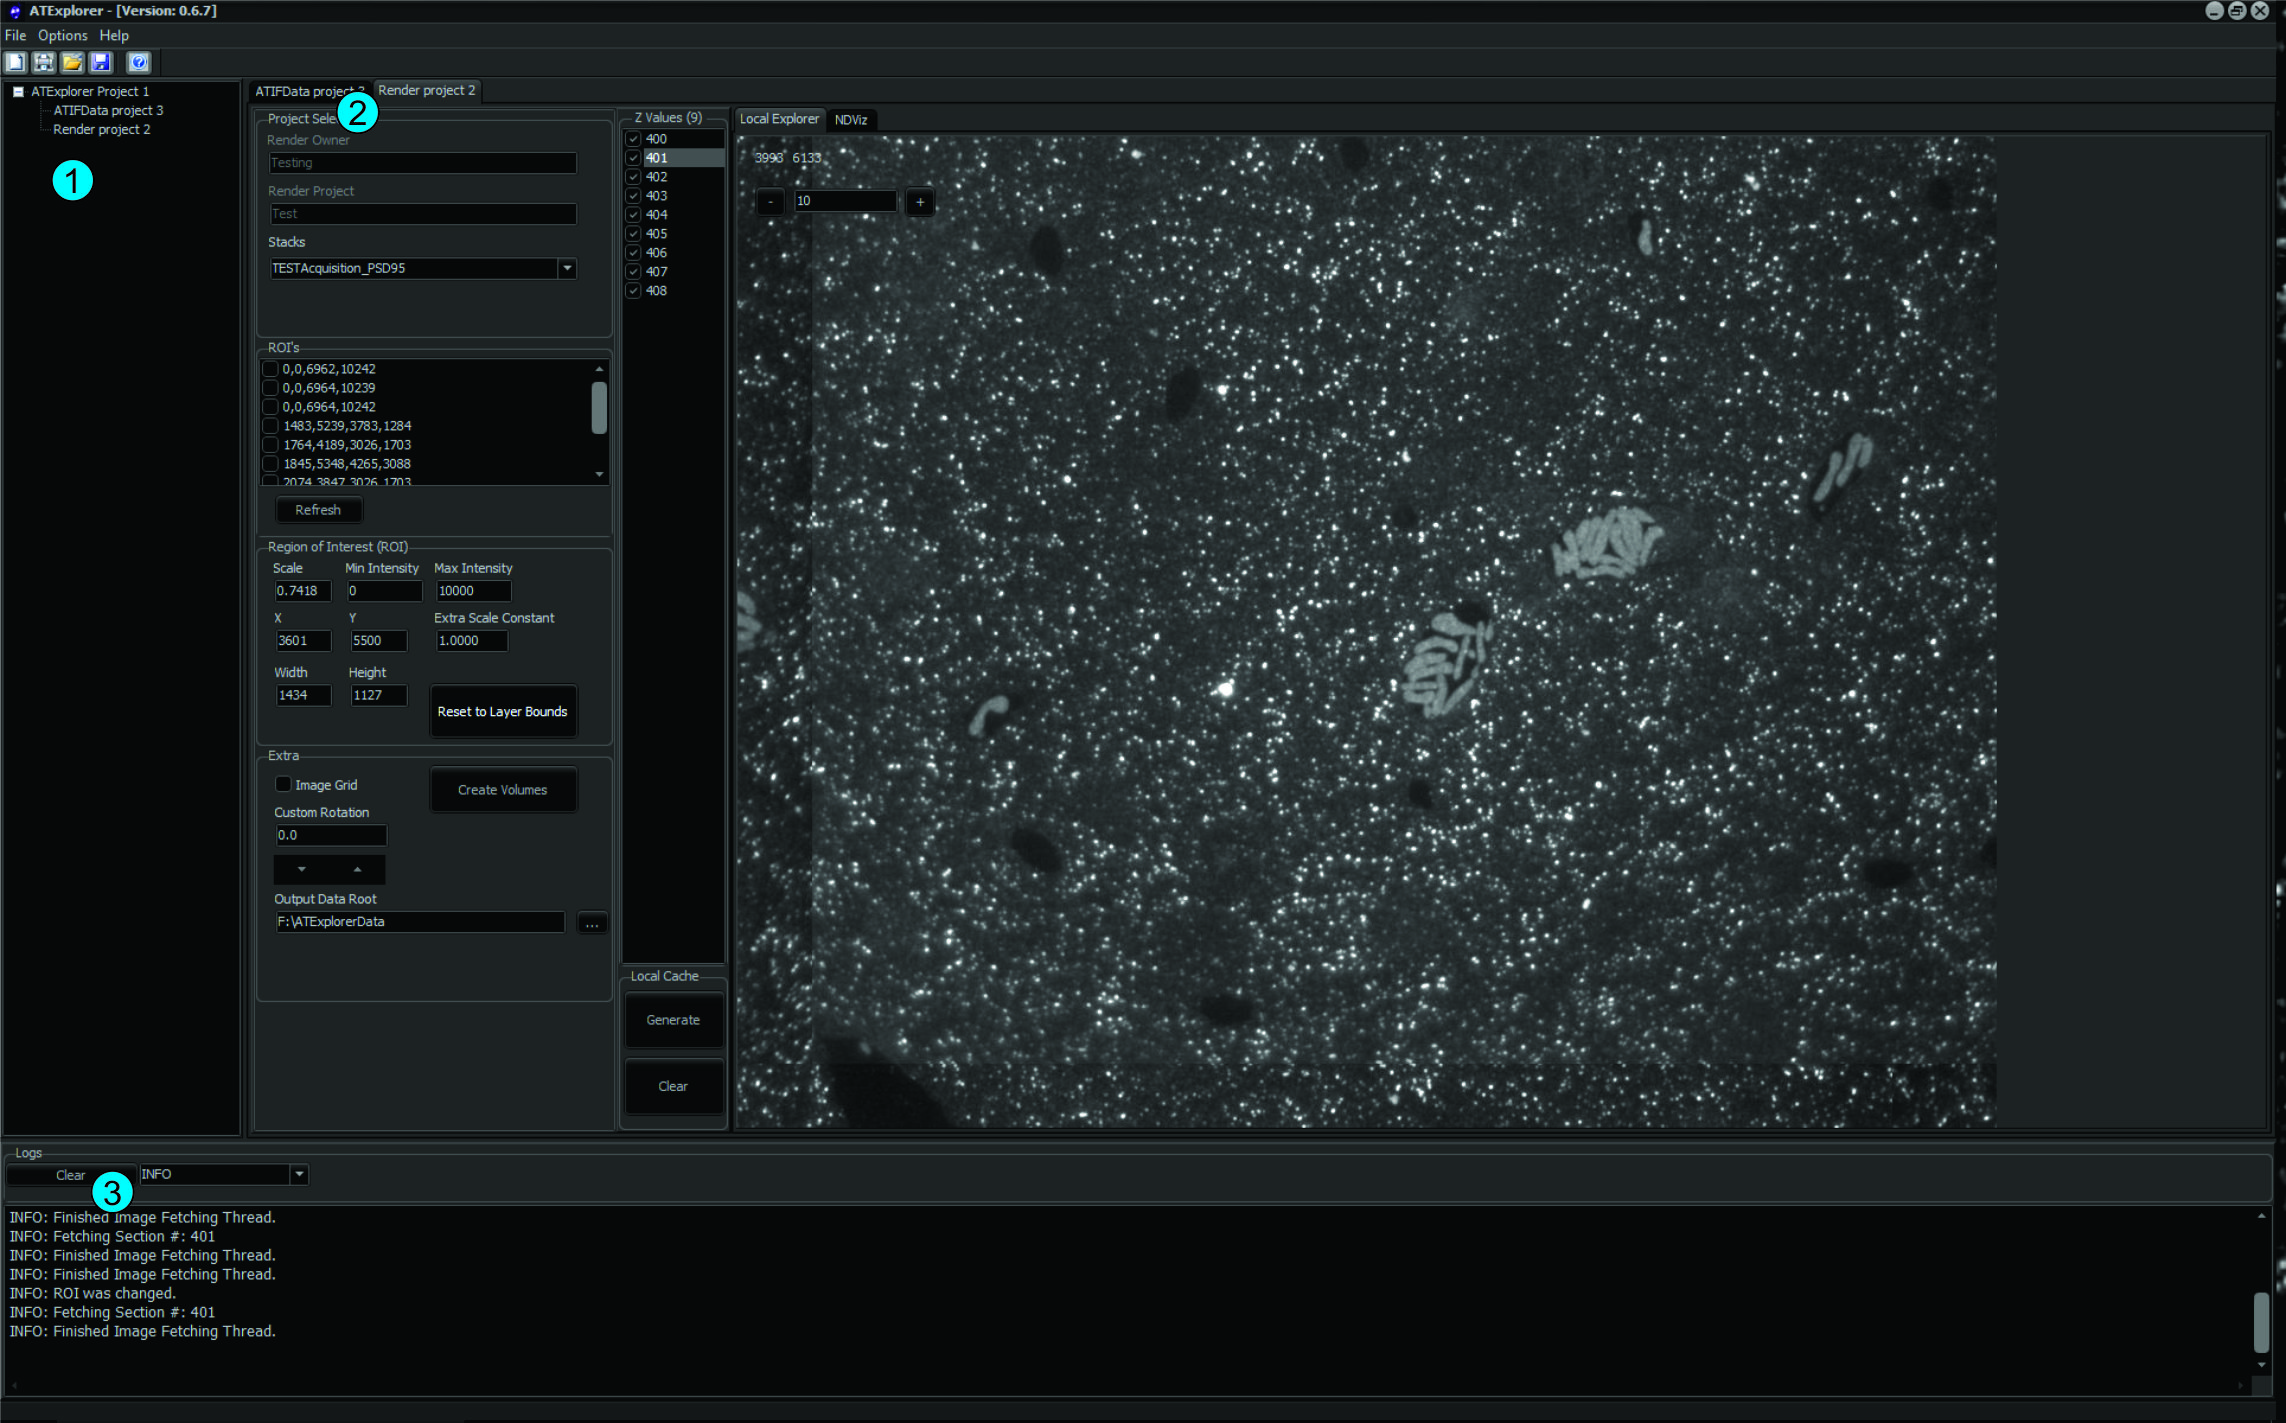
\includegraphics[scale=0.85]{ATExplorerUI_1}

\caption{\ate{} UI. The circled numbers in the figure indicate relevant elements of the UI; \protect\cn{1} Project(s) TreeView. \protect\cn{2} Tabbed Project Item View. \protect\cn{3} Information and Application Log Messages.}
\end{figure}

\subsection{Importing Data}

\begin{description}[font=$\bullet$~\normalfont\scshape\color{red!50!black}]
\item [Importing process] Give an overview on what happens when data is being imported to \ate.
\item [Data Formats] Describe the Allen Institute format, and Kristinas format.
\end{description}

\subsection{Connect to a a Remote (or local) RenderHost}

\subsection{Create of RenderStacks}

\subsection{Manage Stacks in Render}

\subsection{Explore Data}

\section{Python Bindings}